\documentclass[12pt, a4paper]{article}

\usepackage[utf8]{inputenc}
\usepackage{geometry}
\geometry{a4paper, margin=1in}
\usepackage{graphicx}
\usepackage[colorlinks=true, linkcolor=black, urlcolor=primary]{hyperref}
\usepackage{titlesec}
\usepackage{tabularx}
\usepackage{xcolor}
\usepackage{booktabs}
\usepackage{parskip}
\usepackage{longtable}

\definecolor{primary}{RGB}{20, 107, 83}
\definecolor{secondary}{RGB}{200, 200, 200}
\definecolor{graytext}{RGB}{120, 120, 120}

\titleformat{\section}
  {\normalfont\Large\bfseries\color{primary}}
  {\thesection}{1em}{}
  
\titleformat{\subsection}
  {\normalfont\large\bfseries\color{primary}}
  {\thesubsection}{1em}{}

\begin{document}

\begin{titlepage}
    \centering
    \vspace*{2cm}
    
    
\includegraphics[width=5cm]{images/Screenshot 2026-05-21 224726.png}
    
    \vspace{1.5cm}
    
    {\Huge \textbf{\textcolor{primary}{OptiGrid}}} \\
    \vspace{0.5cm}
    {\large \textcolor{graytext}{Energy Intelligence Platform}}
    
    \vspace{2.5cm}
    
    {\Large \textbf{Architectural Requirements}}
    
    \vspace{0.5cm}
    \rule{10cm}{0.4pt}
    
    \vspace{1.5cm}
    
    {\normalsize Version 1.2} \\
    \vspace{0.3cm}
    {\normalsize September 3, 2026}
    
    \vfill
    
    {\normalsize \textbf{Team Coreflow}} \\
    \vspace{0.3cm}
    {\normalsize COS 301 - Capstone Project} \\
    \vspace{0.3cm}
    {\normalsize University of Pretoria}
    
    \vspace*{1cm}
\end{titlepage}

\newpage

\tableofcontents
\newpage

\section{Introduction}
This document outlines the architectural patterns, design choices, system constraints, and the technology stack utilized to keep the platform scalable and secure. The architecture is intentionally designed to support the high throughput of IoT telemetry data while maintaining a responsive and accessible user interface for facility managers.

\section{Architectural Requirements}

\subsection{Architectural Patterns}
OptiGrid uses a hybrid approach, combining \textbf{Microservices} and \textbf{Event-Driven} patterns to ensure the system stays available and scales well under heavy loads.

\begin{itemize}
    \item \textbf{Microservices Architecture:} 
    \begin{itemize}
        \item \textit{Definition:} The system is broken down into smaller, independent services based on what they do (like Data Ingestion, Analytics, and the Dashboard UI), rather than existing as a single monolithic application.
        \item \textit{Justification:} Ingestion traffic can grow separately from dashboard reads. Separate services allow ingestion replicas to be added while the frontend replica count stays fixed, and allow the Python analytics engine to run separately from the Node.js backend. SC01--SC03 test whether independent ingestion scaling meets the workload and dashboard latency targets; separation alone does not establish those performance guarantees.
    \end{itemize}
    \item \textbf{Event-Driven Architecture (EDA):}
    \begin{itemize}
        \item \textit{Definition:} Different parts of the system communicate asynchronously by sending events to a message broker, rather than relying on direct service-to-service calls.
        \item \textit{Justification:} If thousands of IoT meters try to send data at the exact same time, normal API calls would back up and probably crash the database. Using a Redis queue acts as a buffer. The ingestion service drops incoming data onto the queue, which lets the database write it at a safe, steady pace. This helps prevent data loss even if traffic spikes unexpectedly.
    \end{itemize}
    \item \textbf{Layered Architecture:}
    \begin{itemize}
        \item \textit{Definition:} The system logic is split into 4 strictly separated presentation, access, services and databse layers. Thus it is a four-tiered layered architecture
        \item \textit{Justification:} This keeps the codebase highly organized. For example, changing the user interface will not interfere with how data is ingested at the database level, which makes maintaining and updating the system much easier over time.
    \end{itemize}
\end{itemize}

\subsection{Design Patterns}
Several standard design patterns are used in the codebase to keep the system maintainable, modular, and reliable.
\begin{itemize}
    \item \textbf{Model-View-Controller (MVC):}
    \begin{itemize}
        \item \textit{Definition:} Separates the application logic into three interconnected parts to separate internal information from how it is presented to the user.
        \item \textit{Justification:} This is used extensively in the backend services and loosely mirrored in the React frontend. It separates the raw data models from the dashboard views using controllers. This decoupling makes the code significantly easier to test and keeps different concerns clearly separated during development.
    \end{itemize}
    \item \textbf{Singleton Pattern:}
    \begin{itemize}
        \item \textit{Definition:} Restricts a class so it can only be instantiated once globally.
        \item \textit{Justification:} This is used for the database connection pools (PostgreSQL and InfluxDB). Creating a brand new connection for every single request in a busy IoT system would cause massive delays and exhaust the available connections. A Singleton makes sure a single, persistent connection pool is reused efficiently across all incoming requests.
    \end{itemize}
    \item \textbf{Strategy Pattern:}
    \begin{itemize}
        \item \textit{Definition:} A behavioral pattern that lets you select a specific algorithm at runtime from a family of algorithms.
        \item \textit{Justification:} This is used in the Python Analytics engine to pick the right predictive model. The system relies on Optuna to automatically test and choose the best forecasting strategy based on a building's specific energy profile, rather than hardcoding a single, rigid algorithm that might not fit every scenario.
    \end{itemize}
\end{itemize}

\subsection{Constraints}
The architectural choices are shaped by a few strict limitations:
\begin{itemize}
    \item \textbf{Financial \& Infrastructure Constraints:} The project operates under a strict R5000 budget provided by EPI-USE. \textit{Impact:} The project cannot use paid enterprise software or expensive proprietary platforms. The system must stick to open-source tools and use cost-effective cloud options (like AWS Free Tier) to remain financially viable throughout its lifecycle.
    \item \textbf{Hardware \& Data Constraints:} Due to a lack of physical access to real world building smart grids, the system is constrained to supporting simulated telemetry data. \textit{Impact:} The ingestion API has to be flexible enough to take standard JSON payloads over regular HTTPS. It will not be tied to specific hardware protocols; this will make it significantly easier to integrate real-world sensor hardware later on without rewriting the ingestion logic.
    \item \textbf{Deployment Constraints:} The system has to be fully containerised and deployed through an automated CI/CD pipeline, with no manual interventions allowed. \textit{Impact:} Docker must be used for all services. All configuration settings are handled dynamically through \texttt{.env} variables so that the development, staging, and production environments are exactly the same without needing to alter source code.
    \item \textbf{Latency \& Performance Constraints:} Real-time dashboards must reflect data updates in under 2 seconds. \textit{Impact:} A regular relational database cannot handle the heavy write speeds and fast read queries needed for IoT data. The system is forced to use a dedicated Time-Series Database (InfluxDB) that is expressly built for this kind of high-throughput workload.
    \item \textbf{Security \& Regulatory Constraints:} The system handles potentially sensitive building operational data and must adhere strictly to the Protection of Personal Information Act (POPIA). \textit{Impact:} Data has to be encrypted when stored, and strict Role-Based Access Control (RBAC) is needed so users only see their own buildings. The system also has to keep comprehensive audit logs for compliance.
\end{itemize}
 \newpage
\subsection{Architectural Diagram}
Below is the technology-neutral structural blueprint of OptiGrid, illustrating the separation of concerns and data flow.

\begin{center}
    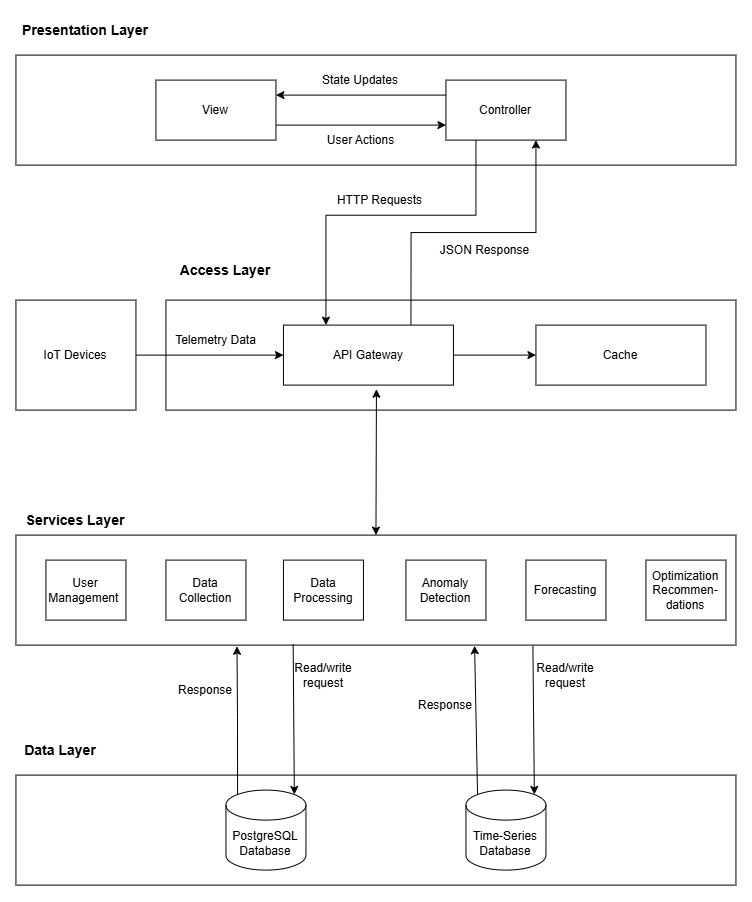
\includegraphics[width=\textwidth]{images/Architecture Diagram.drawio.png}
\end{center}
\newpage
\subsection{Mapping Quality Requirements to Architectural Decisions}
This table maps the quantified Non-Functional Requirements (from the SRS) directly to the architectural mechanisms designed to support their fulfilment.
\begin{table}[h!]
\centering
\sloppy
\renewcommand{\arraystretch}{1.5}
\begin{tabularx}{\textwidth}{|>{\hsize=.3\hsize}X|>{\hsize=.7\hsize}X|}
\hline
\textbf{Quality Requirement (from SRS)} & \textbf{Architectural Mechanism \& Justification} \\ \hline
\textbf{Performance:} Respond to requests within 2 seconds for 95\% of requests. & \textbf{Time-Series Database \& Pre-aggregation:} Using InfluxDB for telemetry makes querying date ranges very fast. Background cron jobs are also used to pre-calculate data into 15-minute and hourly summaries. This means the dashboard only has to load small datasets instead of calculating millions of rows on the fly, keeping load times under a second. \\ \hline
\textbf{Scalability:} Support up to 200\% workload increase with no more than 10\% performance drop. & \textbf{Independent Services, Horizontal Replicas \& Queue Buffering:} Ingestion APIs and workers can be replicated independently of the frontend. SC01--SC04 test load growth, replica distribution, dashboard isolation and queue drainage. SC05 tests an experimental local traffic-driven scaling controller. Docker containers alone do not provide autoscaling; production cloud autoscaling remains unverified. \\ \hline
\textbf{Security:} AES-256 encryption and multi-factor authentication enforcement. & \textbf{Centralised Authentication + TLS 1.3 + JWT:} The authentication layer serves as a strict gateway. All outside traffic is forced to use HTTPS (TLS 1.3), and short-lived JSON Web Tokens (JWTs) are used to safely verify user permissions on every request without storing session data on the server. \\ \hline
\textbf{Reliability:} 99.9\% uptime and recover from critical failures $<$ 5 minutes. & \textbf{Message Broker (Redis Queue) Buffering:} If the main database goes down, the ingestion API will not lose data. Incoming telemetry waits safely in the Redis queue until the database comes back online, preventing data loss while the system automatically recovers. \\ \hline
\textbf{Usability:} Core tasks completed in $<$5 min, 85\% user satisfaction. & \textbf{Dashboard-First MVC UI Design:} Using React along with a robust state management system allows the UI to update instantly without reloading the page. A standard set of design tokens is also used to keep navigation clear and contrast ratios highly accessible for all users. \\ \hline
\textbf{Maintainability:} Cyclomatic complexity $\leq 10$ per application function and at least 80\% automated test coverage. & \textbf{Focused Functions, Separation of Concerns \& Automated Checks:} Layer separation and focused functions are intended to isolate changes and make code easier to test. Executable dependency checks, coverage gates and static complexity analysis verify these claims. Local coverage enforcement has been verified; the existing CI workflow must still invoke these checks before merge enforcement can be claimed. \\ \hline
\end{tabularx}
\end{table}


\newpage
\subsection{Maintainability NFR Traceability}
The maintainability requirement was revised on September 3, 2026: M04 measures
function complexity and replaces the former two-hour deployment target.
The acceptance criterion is a maximum complexity of 10 for each application
function, not an average. The 80\% automated coverage target is retained.
Coverage is measured as line coverage per component for this test plan.

\renewcommand{\arraystretch}{1.3}
\begin{longtable}{|p{0.05\textwidth}|p{0.18\textwidth}|p{0.19\textwidth}|p{0.22\textwidth}|p{0.20\textwidth}|}
\hline
\textbf{ID} & \textbf{Quality target} & \textbf{Architectural tactic} & \textbf{Executable test and criterion} & \textbf{Evidence and result} \\ \hline
\endfirsthead
\hline
\textbf{ID} & \textbf{Quality target} & \textbf{Architectural tactic} & \textbf{Executable test and criterion} & \textbf{Evidence and result} \\ \hline
\endhead
M01 & At least 80\% automated coverage. & Automated unit testing and testable components. & Run Jest and pytest-cov over all scoped source. All tests pass and each component reaches 80\% line coverage. & Coverage reports: frontend 70.39\%, core 74.12\%, ingestion 44.49\%, analytics 80.50\%. Overall FAIL. \\ \hline
M02 & Maintain separation of concerns. & Layered architecture, MVC and independent services. & Parse source dependencies against documented layer rules. Zero forbidden imports or analysis errors; checker fixtures pass. & Dependency reports: 185 files, zero violations, 6 checker fixtures pass. PASS within documented scope. \\ \hline
M03 & Enforce the 80\% coverage threshold. & Automated quality checks. & Test low-coverage and passing fixtures with the shared threshold. Low coverage must cause a nonzero exit; full coverage must pass. & Jest and pytest-cov both reject 37.50\% and accept 100\%. Local PASS; CI wiring and required merge checks remain unverified. \\ \hline
M04 & Complexity $\leq 10$ per application function. & Small, focused functions and separation of responsibilities. & Run ESLint complexity analysis and Radon with boundary fixtures. Zero functions above 10 and zero analysis errors. & 1,248 functions checked; 41 exceed 10. All 11 analyzer fixtures pass. Overall FAIL; ingestion passes. \\ \hline
M05 & Maintain code quality and buildability. & Static analysis and automated builds. & Run existing lint rules on authored source and the normal production builds. Zero lint errors; both builds succeed. & Zero lint errors, 23 warnings; both builds succeed. PASS with warnings. \\ \hline
\end{longtable}

Run the tests from the repository root using:
\begin{verbatim}
node scripts/nfr-maintainability.mjs
node scripts/nfr-maintainability.mjs --only m04
\end{verbatim}

Test scope and tool versions are documented in
\path{tests/nfr/maintainability/README.md}. M04 excludes test fixtures, generated
code, declarations and third-party dependencies, and includes callbacks, methods,
nested functions and Python lambdas. ESLint 8.57.1 and Radon 6.0.1 provide the
versioned counting conventions. Complexity is one indicator of maintainability;
the dependency, coverage and build checks provide complementary evidence.

The measured results and artifact links are in
\path{docs/testing/maintainability-results-2026-09-03.md}. Raw reports include the
source commit, commands, timestamps, per-function scores and pass/fail outcomes.
The local checks do not require an AWS deployment. Failed thresholds remain
unchanged while the implementation is improved and retested.

\newpage
\subsection{Scalability NFR Traceability}
The SRS scalability target is retained: a workload increase of up to 200\%,
without major architectural changes or more than a 10\% performance decrease.
For this local test plan, the operational baseline is $W=50$ telemetry requests
per second across 100 buildings. A 200\% increase means $3W=150$ requests per
second. Performance is measured as HTTP p95 latency, with elevated-load p95 at
most $1.10$ times baseline and request errors below 1\%. These definitions make
the SRS executable; they are not claims that it already specifies this workload.

Sustained scenarios have 30 seconds of warm-up and five measured minutes.
The generator must deliver the requested rate within 1\%, with p95 scheduling
lag at most 100 ms. Every acknowledged telemetry key, including warm-up, must
be present in InfluxDB and the queue empty within 120 seconds after load stops.
The frontend and core each remain at one replica; ingestion APIs and workers
scale together. Thresholds were fixed before execution.
Latency and error criteria use the measured window. SC05's warm-up failures
are reported separately and must be considered before claiming uninterrupted
service during scaling.

\renewcommand{\arraystretch}{1.3}
\begin{longtable}{|p{0.05\textwidth}|p{0.18\textwidth}|p{0.19\textwidth}|p{0.22\textwidth}|p{0.20\textwidth}|}
\hline
\textbf{ID} & \textbf{Quality target} & \textbf{Architectural tactic} & \textbf{Executable test and criterion} & \textbf{Evidence and result} \\ \hline
\endfirsthead
\hline
\textbf{ID} & \textbf{Quality target} & \textbf{Architectural tactic} & \textbf{Executable test and criterion} & \textbf{Evidence and result} \\ \hline
\endhead
SC01 & Support $W$, $2W$, $3W$ within the latency/error limits. & Independent services and horizontal ingestion replicas. & Run 50/s with one replica, 100/s with two, 150/s with three. Both elevated p95 ratios $\leq1.10$; validate errors, delivered rate and persistence. & FAIL. p95 at W/2W/3W: 34.17/36.33/51.18 ms. Limit 37.58 ms. \\ \hline
SC02 & Meet the elevated workload by scaling ingestion. & Replicated APIs, load distribution and concurrent workers. & Compare 150/s with one versus three replicas. Three must meet SC01 criteria; all three APIs and workers must process data. & FAIL. At 150/s, p95 one/three replicas: 85.91/51.18 ms. Per-replica traffic and writes saved. \\ \hline
SC03 & Preserve dashboard API responsiveness during ingestion growth. & Separate frontend/core and ingestion services. & Read live telemetry at 2/s under $W$ and $3W$. Validate 100 building rows; read p95 ratio $\leq1.10$, errors $<1\%$, one frontend throughout. & FAIL. Read p95: 25.87 to 43.87 ms; limit 28.46 ms. \\ \hline
SC04 & Buffer a temporary telemetry burst without missing accepted points. & Redis queue and asynchronous workers. & Send 150/s for 60 seconds. Errors $<1\%$, valid generator, zero missing/unexpected keys and queue drained within 120 seconds. & PASS. 9000/9000 accepted, 0 missing; drain verified in 0.12 s. \\ \hline
SC05 & Respond automatically to measured local load. & Experimental traffic-driven controller and Docker replicas. & At 150/s, measured rate $\geq100$/s sustained for 10 seconds triggers scaling from one to three. Ready within 60 seconds; meet SC01 traffic/persistence limits. & FAIL under local criteria. Ready in 9.48 s; p95 52.06 ms. Warm-up write errors: 474. \\ \hline
\end{longtable}

Run the local suite from the repository root using:
\begin{verbatim}
node scripts/nfr-scalability.mjs --mode preflight
node scripts/nfr-scalability.mjs
\end{verbatim}

The protocol, resource limits and setup are in
\path{tests/nfr/scalability/README.md}. The measured results and evidence links
are in \path{docs/testing/scalability-results-2026-09-03.md}. Evidence includes
request-level traces, queue samples, accepted/stored point reconciliation,
replica topology, worker activity, resource use and controller events.

\textbf{Scope:} All results are from an isolated local Docker configuration
while the normal OptiGrid stack remained running. The real frontend/core
live-telemetry API and ingestion-to-InfluxDB path were exercised. Browser
rendering, authenticated metadata operations, unrelated scheduled jobs,
production TLS overhead, AWS capacity and production autoscaling were not
tested. SC04 covers burst buffering with healthy dependencies, not persistence
during dependency failures. SC05 is a local prototype, not a deployed cloud
controller. Failed criteria remain failures until the tactic is improved and
the unchanged test plan is rerun.

\newpage
\section{Technology Requirements}

The following technology stack was selected to balance handling lots of data, running machine learning predictions, and building the UI quickly.

\sloppy
\renewcommand{\arraystretch}{1.5}
\begin{longtable}{|>{\bfseries}p{0.28\textwidth}|>{\bfseries}p{0.25\textwidth}|p{0.38\textwidth}|}
\hline
\textbf{Component} & \textbf{Selected Technology} & \textbf{Justification} \\ \hline
\endfirsthead
\hline
\textbf{Component} & \textbf{Selected Technology} & \textbf{Justification} \\ \hline
\endhead
Frontend &
React.js &
React is great for building interactive, data-heavy dashboards. Its virtual DOM is fast enough to update complex graphs in real time without lagging. It also has a huge community, making it easy to drop in charting libraries (like Recharts or Chart.js) for the energy graphs. \\ \hline
Backend API &
Node.js    (Express) &
The main challenge for OptiGrid's backend is handling thousands of small API requests at the same time. Node.js uses an event loop that does not block other processes, making it much better at handling high volumes of concurrent connections than traditional multi-threaded languages. \\ \hline
Relational Database &
PostgreSQL  (Supabase) &
This is only used for system metadata (like user profiles, building configs, and permissions). PostgreSQL is reliable, handles complex table joins well, and ensures data stays strictly isolated between different tenants. \\ \hline
Time-Series Database &
InfluxDB &
Trying to store millions of telemetry data points in a standard SQL database usually ruins indexing performance over time. InfluxDB is specifically designed for time-stamped data, allowing for fast writes and easy automatic data downsampling. \\ \hline
Analytics Engine &
Python (scikit-learn, Pandas, Optuna) &
Python is the standard choice for data science. Using libraries like scikit-learn, Pandas, and Optuna allows the system to efficiently predict future demand based on historical data. Putting this in its own Python microservice allows the use of the best machine learning tools without bloating the Node.js backend. \\ \hline
Containerisation &
Docker &
Docker solves the "it works on my machine" problem. It ensures that the code runs exactly the same way on a developer's laptop, in the development environment, and on the AWS cloud servers. \\ \hline
Hosting &
AWS (Backend), Vercel (Frontend) &
AWS allows us to host the backend services on a live platform, it makes it easy for us to deploy our system since we use Docker. Vercel hosts our frontend and speaks to AWS for any requests to fetch data. Vercel creates pre-production environments so we can see how our app looks with code changes before pushing to the production environment. \\ \hline
\end{longtable}
\newpage
\section{API Contracts}

\subsection{Authentication}
\begin{enumerate}
    \item \textbf{signup}
    \begin{itemize}
        \item POST 
        \item \textbf{Request:}
        \begin{verbatim}
{
    email: string,
    password: string,
    name: string
}
        \end{verbatim}
        Example:
        \begin{verbatim}
{
    "email": "user@example.com",
    "password": "SecurePass123!",
    "name": "John Doe"
}
        \end{verbatim}
        \item \textbf{Response:}
        \begin{verbatim}
{
    "message": "User created successfully",
    "user": {
        "userId": "123e4567-e89b-12d3-a456-426614174000",
        "email": "user@example.com",
        "firstName": "John",
        "lastName": "Doe"
    }
}
        \end{verbatim}
        \item \textbf{Effect:}
        \begin{itemize}
            \item Creates a new user.
        \end{itemize}
    \end{itemize}
    \item \textbf{login}
    \begin{itemize}
        \item POST 
        \item \textbf{Request:}
        \begin{verbatim}
{
    email: string,
    password: string
}
        \end{verbatim}
        Example:
        \begin{verbatim}
{
    "email": "user@example.com",
    "password": "SecurePass123!"
}
        \end{verbatim}
        \item \textbf{Response:}
        \begin{verbatim}
{
    "message": "Login successful",
    "user": {
        "userId": "123e4567-e89b-12d3-a456-426614174000",
        "email": "user@example.com",
        "firstName": "John",
        "lastName": "Doe",
        "token": "eyJhbGciOiJIUzI1NiIsInR..."
    }
}
        \end{verbatim}
        \item \textbf{Effect:}
        \begin{itemize}
            \item Authenticates a user with their email and password.
            \item Returns user information along with a JWT token which expires after some time.
        \end{itemize}
    \end{itemize}
    \end{enumerate}
    
\subsection{User Access Control}
\begin{enumerate}
    \item \textbf{getViewers}
    \begin{itemize}
        \item GET
        \item \textbf{Request:} None
        Example:
        \begin{verbatim}
GET /auth/viewers
        \end{verbatim}
        \item \textbf{Response:}
        \begin{verbatim}
{
    "data": [
        {
            "userId": "123e4567-e89b-12d3-a456-426614174000",
            "email": "viewer@example.com",
            "firstName": "Jane",
            "lastName": "Smith",
            "roleType": "VIEWER",
            "buildingIds": ["uuid-1", "uuid-2"]
        }
    ]
}
        \end{verbatim}
        \item \textbf{Effect:}
        \begin{itemize}
            \item Fetches all users with the VIEWER role and their assigned building IDs.
            \item Requires ADMIN access.
        \end{itemize}
    \end{itemize}
    \item \textbf{getManagers}
    \begin{itemize}
        \item GET 
        \item \textbf{Request:} None
        Example:
        \begin{verbatim}
GET /auth/managers
        \end{verbatim}
        \item \textbf{Response:}
        \begin{verbatim}
{
    "data": [
        {
            "userId": "123e4567-e89b-12d3-a456-426614174000",
            "email": "manager@example.com",
            "firstName": "Mark",
            "lastName": "Johnson",
            "roleType": "BUILDING_MANAGER",
            "buildingIds": ["uuid-1"]
        }
    ]
}
        \end{verbatim}
        \item \textbf{Effect:}
        \begin{itemize}
            \item Fetches all users with the BUILDING\_MANAGER role and their assigned building IDs.
            \item Requires ADMIN access.
        \end{itemize}
    \end{itemize}
    \item \textbf{assignManager}
    \begin{itemize}
        \item POST 
        \item \textbf{Request:}
        \begin{verbatim}
{
    userId: string,
    buildingId: string
}
        \end{verbatim}
        Example:
        \begin{verbatim}
{
    "userId": "123e4567-e89b-12d3-a456-426614174000",
    "buildingId": "888e4567-e89b-12d3-a456-426614174000"
}
        \end{verbatim}
        \item \textbf{Response:}
        \begin{verbatim}
{
    "success": true,
    "message": "Manager assigned to building successfully"
}
        \end{verbatim}
        \item \textbf{Effect:}
        \begin{itemize}
            \item Assigns a building manager to a specific building.
            \item Requires ADMIN access.
        \end{itemize}
    \end{itemize}
    \item \textbf{removeManager}
    \begin{itemize}
        \item DELETE
        \item \textbf{Request:}
        \begin{verbatim}
{
    userId: string,
    buildingId: string
}
        \end{verbatim}
        Example:
        \begin{verbatim}
{
    "userId": "123e4567-e89b-12d3-a456-426614174000",
    "buildingId": "888e4567-e89b-12d3-a456-426614174000"
}
        \end{verbatim}
        \item \textbf{Response:}
        \begin{verbatim}
{
    "success": true,
    "message": "Manager removed from building successfully"
}
        \end{verbatim}
        \item \textbf{Effect:}
        \begin{itemize}
            \item Removes a manager's access from a specific building.
            \item Requires ADMIN access.
        \end{itemize}
    \end{itemize}
\end{enumerate}

\subsection{Buildings}
\begin{enumerate}
    \item \textbf{getAllBuildings}
    \begin{itemize}
        \item GET
        \item \textbf{Request:}
        \begin{verbatim}
Query Parameters:
    lifecycle_state: string (optional)
        \end{verbatim}
        Example:
        \begin{verbatim}
GET /admin?lifecycle_state=ACTIVE
        \end{verbatim}
        \item \textbf{Response:}
        \begin{verbatim}
{
    "status": "success",
    "data": [
        {
            "building_id": "123e4567-e89b-12d3-a456-426614174000",
            "building_name": "Main Campus",
            "building_type": "EDUCATIONAL",
            "lifecycle_state": "ACTIVE"
        }
    ]
}
        \end{verbatim}
        \item \textbf{Effect:}
        \begin{itemize}
            \item Fetches all buildings that are in the database.
            \item Requires ADMIN access.
        \end{itemize}
    \end{itemize}
    \item \textbf{getManagerBuildings}
    \begin{itemize}
        \item GET 
        \item \textbf{Request:} None
        Example:
        \begin{verbatim}
GET /manager
        \end{verbatim}
        \item \textbf{Response:}
        \begin{verbatim}
{
    "status": "success",
    "data": [
        {
            "building_id": "123e4567-e89b-12d3-a456-426614174000",
            "building_name": "Science Block",
            "todays_usage": 152.4
        }
    ]
}
        \end{verbatim}
        \item \textbf{Effect:}
        \begin{itemize}
            \item Fetches all buildings assigned to the currently authenticated manager.
        \end{itemize}
    \end{itemize}
    \item \textbf{createBuilding}
    \begin{itemize}
        \item POST 
        \item \textbf{Request:}
        \begin{verbatim}
Headers:
    idempotency-key: string
Body:
{
    building_name: string,
    building_type: string,
    square_footage?: number,
    timezone?: string,
    max_occupancy?: number,
    physical_address?: string,
    latitude?: number,
    longitude?: number,
    geohash?: string
}
        \end{verbatim}
        Example:
        \begin{verbatim}
POST /api/buildings
Headers: { "idempotency-key": "550e8400-e29b-41d4-a716-446655440000" }
{
    "building_name": "Corporate Headquarters",
    "building_type": "OFFICE",
    "square_footage": 75000,
    "physical_address": "123 Main Street"
}
        \end{verbatim}
        \item \textbf{Response:}
        \begin{verbatim}
{
    "status": "success",
    "data": {
        "id": "123e4567-e89b-12d3-a456-426614174000",
        "building_name": "Corporate Headquarters",
        "building_type": "OFFICE"
    }
}
        \end{verbatim}
        \item \textbf{Effect:}
        \begin{itemize}
            \item Creates a new building with the provided details.
            \item Uses an idempotency key to prevent duplicate requests.
            \item The building is created in 'PROVISIONING' state by default.
        \end{itemize}
    \end{itemize}
    \item \textbf{getBuildingDetails}
    \begin{itemize}
        \item GET
        \item \textbf{Request:}
        \begin{verbatim}
Path Parameters:
    building_id: string
        \end{verbatim}
        Example:
        \begin{verbatim}
GET /api/buildings/123e4567-e89b-12d3-a456-426614174000
        \end{verbatim}
        \item \textbf{Response:}
        \begin{verbatim}
{
    "status": "success",
    "data": {
        "building_id": "123e4567-e89b-12d3-a456-426614174000",
        "building_name": "Corporate Headquarters",
        "timezone": "Africa/Johannesburg"
    }
}
        \end{verbatim}
        \item \textbf{Effect:}
        \begin{itemize}
            \item Returns all relevant details for a single building including.
            \item Only accessible if the authenticated user has access to it.
        \end{itemize}
    \end{itemize}
    \item \textbf{getBuildingEnergyConsumption}
    \begin{itemize}
        \item GET 
        \item \textbf{Request:}
        \begin{verbatim}
Path Parameters:
    building_id: string
Query Parameters:
    time_range: string (e.g., '7d', '30d')
        \end{verbatim}
        Example:
        \begin{verbatim}
GET /api/buildings/123e4567-e89b-12d3-a456-426614174000/energy-consumption?time_range=30d
        \end{verbatim}
        \item \textbf{Response:}
        \begin{verbatim}
{
    "status": "success",
    "data": {
        "building_id": "123e4567-e89b-12d3-a456-426614174000",
        "total_kwh": 1234.56,
        "average_daily_kwh": 41.15,
        "cost_per_kwh": 2.5
    }
}
        \end{verbatim}
        \item \textbf{Effect:}
        \begin{itemize}
            \item Returns energy consumption metrics for a single building over a selected time range.
        \end{itemize}
    \end{itemize}
    \item \textbf{updateBuilding}
    \begin{itemize}
        \item PATCH 
        \item \textbf{Request:}
        \begin{verbatim}
Path Parameters:
    building_id: string
Body:
{
    building_name?: string,
    building_type?: string,
    square_footage?: number,
    timezone?: string,
    max_occupancy?: number,
    physical_address?: string
}
        \end{verbatim}
        Example:
        \begin{verbatim}
PATCH /api/buildings/123e4567-e89b-12d3-a456-426614174000
{
    "building_name": "Renamed Corporate Office"
}
        \end{verbatim}
        \item \textbf{Response:}
        \begin{verbatim}
{
    "status": "success",
    "data": { ...updated_building_details... }
}
        \end{verbatim}
        \item \textbf{Effect:}
        \begin{itemize}
            \item Updates specific properties of a building.
            \item Requires ADMIN or MANAGER access.
        \end{itemize}
    \end{itemize}
    \item \textbf{deleteBuilding}
    \begin{itemize}
        \item DELETE
        \item \textbf{Request:}
        \begin{verbatim}
Path Parameters:
    building_id: string
        \end{verbatim}
        Example:
        \begin{verbatim}
DELETE /api/buildings/123e4567-e89b-12d3-a456-426614174000
        \end{verbatim}
        \item \textbf{Response:}
        \begin{verbatim}
{
    "status": "success",
    "message": "Building successfully deleted"
}
        \end{verbatim}
        \item \textbf{Effect:}
        \begin{itemize}
            \item  Removes a building from the database.
            \item Requires ADMIN access
        \end{itemize}
    \end{itemize}
    \item \textbf{compareBuildings}
    \begin{itemize}
        \item POST 
        \item \textbf{Request:}
        \begin{verbatim}
Headers:
    idempotency-key: string
Query Parameters:
    buildingID_1: string
    buildingID_2: string
    time_range: string (e.g., '30d')
        \end{verbatim}
        Example:
        \begin{verbatim}
POST /api/buildings/compare?buildingID_1=uuid1&buildingID_2=uuid2&time_range=30d
Headers: { "idempotency-key": "660e8400-e29b-41d4-a716-446655440001" }
        \end{verbatim}
        \item \textbf{Response:}
        \begin{verbatim}
{
    "status": "success",
    "data": {
        "building_a": { "energy_consumption": 1500, "cost": 3000 },
        "building_b": { "energy_consumption": 1200, "cost": 2400 },
        "comparison": { ... }
    }
}
        \end{verbatim}
        \item \textbf{Effect:}
        \begin{itemize}
            \item Compares energy consumption and performance metrics between two chosen buildings for a given time range.
        \end{itemize}
    \end{itemize}
\end{enumerate}

\subsection{Preferences}
\begin{enumerate}
    \item \textbf{getUserTheme}
    \begin{itemize}
        \item GET 
        \item \textbf{Request:} None
        Example:
        \begin{verbatim}
GET /api/preferences/theme
        \end{verbatim}
        \item \textbf{Response:}
        \begin{verbatim}
{
    "theme": "dark"
}
        \end{verbatim}
        \item \textbf{Effect:}
        \begin{itemize}
            \item Retrieves the current user's theme preference (light, dark, or system).
        \end{itemize}
    \end{itemize}
    \item \textbf{updateUserTheme}
    \begin{itemize}
        \item PUT 
        \item \textbf{Request:}
        \begin{verbatim}
{
    theme: "light" | "dark" | "system"
}
        \end{verbatim}
        Example:
        \begin{verbatim}
PUT /api/preferences/theme
{
    "theme": "light"
}
        \end{verbatim}
        \item \textbf{Response:}
        \begin{verbatim}
200 OK (Preference updated)
        \end{verbatim}
        \item \textbf{Effect:}
        \begin{itemize}
            \item Updates the current user's theme preference in the database.
        \end{itemize}
    \end{itemize}
\end{enumerate}
\subsection{Analytics}
\begin{enumerate}
    \item \textbf{getForecast}
    \begin{itemize}
        \item POST 
        \item \textbf{Request:}
        \begin{verbatim}
Path Parameters:
    building_id: string
Body:
{
    horizon_days: number,
    granularity: string
}
        \end{verbatim}
        Example:
        \begin{verbatim}
POST /api/analytics/forecast/123e4567-e89b-12d3-a456-426614174000
{
    "horizon_days": 7,
    "granularity": "hourly"
}
        \end{verbatim}
        \item \textbf{Response:}
        \begin{verbatim}
{
    "historical": [ ... ],
    "forecast": [ ... ],
    "summary": { ... }
}
        \end{verbatim}
        \item \textbf{Effect:}
        \begin{itemize}
            \item Calculates an energy usage forecast graph for a specific building based on historical data.
        \end{itemize}
    \end{itemize}
\end{enumerate}

\subsection{Sensors}
\begin{enumerate}
    \item \textbf{handleSensorTelemetry}
    \begin{itemize}
        \item POST
        \item \textbf{Request:}
        \begin{verbatim}
{
    building_id: string,
    sensor_id: string,
    usage: number,
    timestamp?: string
}
        \end{verbatim}
        Example:
        \begin{verbatim}
POST /api/sensors/data
{
    "building_id": "building-001",
    "sensor_id": "sensor-001",
    "usage": 12.34
}
        \end{verbatim}
        \item \textbf{Response:}
        \begin{verbatim}
{
    "status": "success"
}
        \end{verbatim}
        \item \textbf{Effect:}
        \begin{itemize}
            \item Submit telemtery data to sensors securely.
        \end{itemize}
    \end{itemize}
    \item \textbf{listSensors}
    \begin{itemize}
        \item GET 
        \item \textbf{Request:}
        \begin{verbatim}
Query Parameters:
    building_id: string
        \end{verbatim}
        Example:
        \begin{verbatim}
GET /api/sensors?building_id=123e4567-e89b-12d3-a456-426614174000
        \end{verbatim}
        \item \textbf{Response:}
        \begin{verbatim}
[
    {
        "id": "sensor-001",
        "mac_address": "AA:BB:CC:DD:EE:FF",
        "status": "Active"
    }
]
        \end{verbatim}
        \item \textbf{Effect:}
        \begin{itemize}
            \item Returns every sensor registered to the given building.
            \item Allowed for any authenticated user with access to the building.
        \end{itemize}
    \end{itemize}
    \item \textbf{registerSensor}
    \begin{itemize}
        \item POST 
        \item \textbf{Request:}
        \begin{verbatim}
{
    building_id: string,
    mac_address: string,
    sensor_type: string,
    unit: string,
    location_zone: string,
    status: string
}
        \end{verbatim}
        Example:
        \begin{verbatim}
POST /api/sensors
{
    "building_id": "123e4567-e89b-12d3-a456-426614174000",
    "mac_address": "AA:BB:CC:DD:EE:FF",
    "sensor_type": "Energy meter",
    "unit": "kWh",
    "location_zone": "Main incomer",
    "status": "Active"
}
        \end{verbatim}
        \item \textbf{Response:}
        \begin{verbatim}
201 Created (Sensor registered successfully)
        \end{verbatim}
        \item \textbf{Effect:}
        \begin{itemize}
            \item Registers a new sensor for the specified building. 
            \item Requires ADMIN and MANAGER access.
        \end{itemize}
    \end{itemize}
    \item \textbf{deleteSensor}
    \begin{itemize}
        \item DELETE
        \item \textbf{Request:}
        \begin{verbatim}
Path Parameters:
    sensor_id: string
        \end{verbatim}
        Example:
        \begin{verbatim}
DELETE /api/sensors/sensor-001
        \end{verbatim}
        \item \textbf{Response:}
        \begin{verbatim}
200 OK (Sensor deleted successfully)
        \end{verbatim}
        \item \textbf{Effect:}
        \begin{itemize}
            \item Deletes the sensor from its building.
            \item Requires ADMIN and MANAGER access.
        \end{itemize}
    \end{itemize}
\end{enumerate}


\newpage
\section{Deployment}

Deployment refers to publishing and running the software system in an accessible environment so that users, clients, and evaluators can interact with it without requiring local installation.

\subsection{Deployment Requirements}

\subsubsection{Live, Accessible System}

Optigrid is deployed and accessible via the link in the root README. The frontend is accesible via the public url which connects to the backend hosted on AWS whichis only accessible to team members.

\subsubsection{Environment Parity}

The system distinguishes between development and production environments. The main branch automatically deploys to at least one non-local environment using the Vercel configurations. 
Development is managed locally via Docker commands and Supabase CLI or Supabase web editor to replicate prodcution database.
Production: Automatically deployed when develop is merged into main branch.

\subsubsection{Infrastructure as Code (IaC) / Containerisation}

The complete system is deployable through Docker and Docker Compose, ensuring deployments are reproducible across environments. No manual deployment steps ("click-ops") are required.

Containerisation: All backend and frontend services are containerised using optimised Dokcerfiles available in their respective folders.
IAC: AWS resources are provisioned using Terraform and are controlled.

\subsubsection{Secrets Management}

All environment variables are put in a .gitnore file.
They are stored securely using Github Secrets and Vercel/AWS Parameter Store. 

\subsubsection{Rollback Strategy}

To ensure rapid recovery from deployment failure we implement a multi-tiered rollback poliicies: 
1. Container Image Tagging: Docker images in production are tagged with release commit hash alongside latest. If a deployment fails, the docker containers are revereted to the previously working version ensuring rapid recovery.
2. Frontend Instant Rollback: Vercel deployment allow instant 1-click rollbacks to the last knonw stable frontend deployment if the frontend fails with new code.

\subsection{Deployment Diagrams}

The following diagrams illustrate where the system is deployed and how software changes move through the deployment pipeline.

\end{document}
